% ---------------- Retrospectivas ----------------
\section{Retrospectivas}

\subsection{Retrospectivas}

\begin{itemize}
  \item \textbf{Pontos de atenção}:
  \begin{itemize}
    \item Baixa adesão às reuniões intermediárias dificultou o alinhamento.
    \item Houve confusão inicial sobre critérios para selecionar artigos relevantes.
  \end{itemize}

  \item \textbf{O que pode ser melhorado}:
  \begin{itemize}
    \item Criar lembretes automáticos das reuniões.
    \item Alinhar expectativas sobre participação mínima esperada de cada integrante.
  \end{itemize}

  \item \textbf{O que manter/continuar}:
  \begin{itemize}
    \item Organização via checklist e Kanban funcionou bem.
    \item Leitura coletiva de fontes-chave ajudou a focar na qualidade da bibliografia.
  \end{itemize}
\end{itemize}

\vspace{1em}
\noindent\textbf{Burndown Chart:}

\begin{center}
  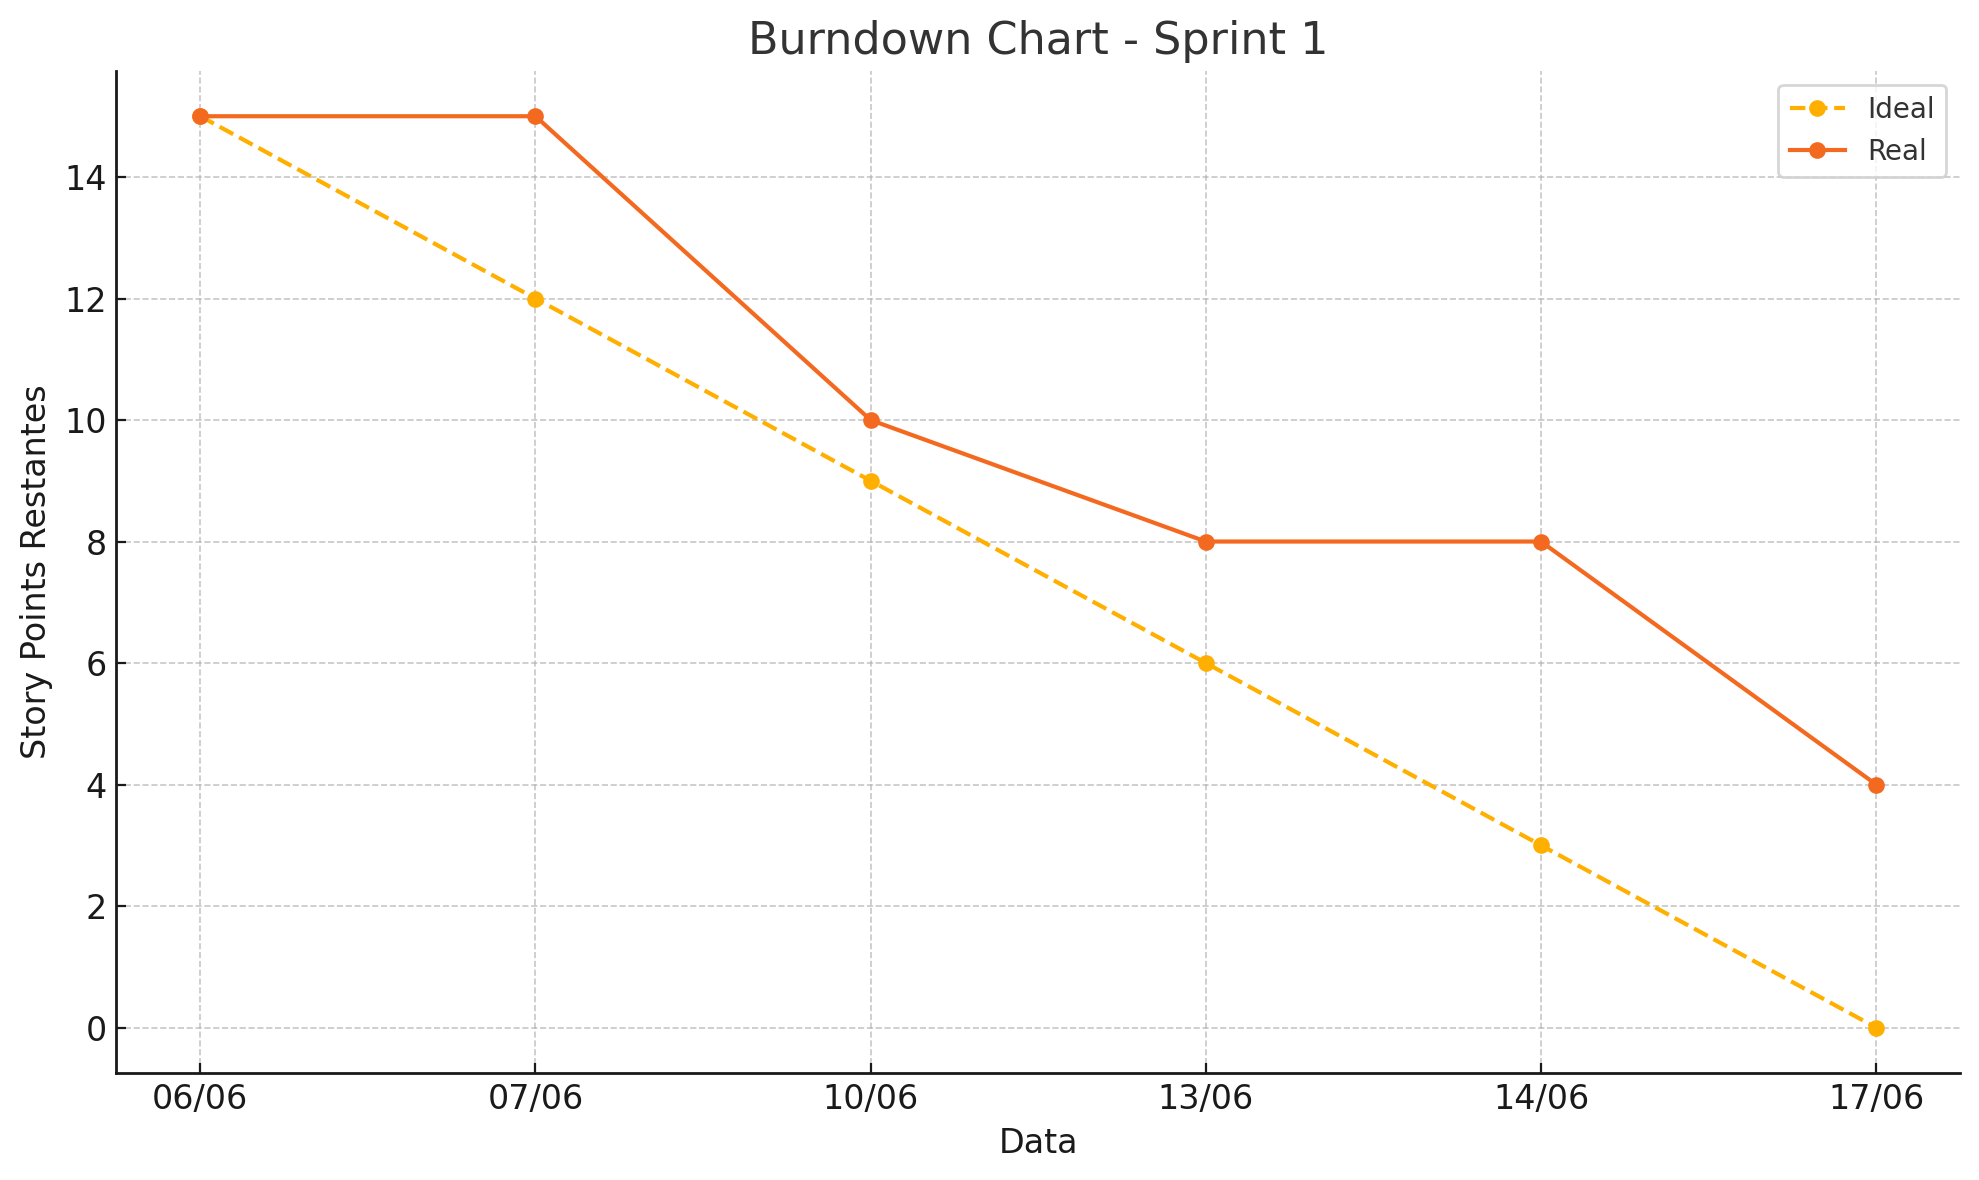
\includegraphics[width=0.8\textwidth]{pictures/burndown_sprint1.png}
\end{center}

\subsection{Retrospectivas}

\begin{itemize}
  \item \textbf{Pontos de atenção}:
  \begin{itemize}
    \item Houve apenas uma daily.
    \item O escopo da sprint foi subdimensionado: todas as tarefas foram concluídas rapidamente, sugerindo que seria possível incluir mais atividades.
  \end{itemize}

  \item \textbf{O que pode ser melhorado}:
  \begin{itemize}
    \item Garantir acompanhamento contínuo (respeitar as dailies).
    \item Refinar o planejamento de sprint com base na capacidade real do grupo, prevendo mais tarefas quando possível.
  \end{itemize}

  \item \textbf{O que manter/continuar}:
  \begin{itemize}
    \item Boa execução e comprometimento da equipe com as entregas.
    \item Clareza nos objetivos da sprint facilitou o foco e a conclusão eficiente das tarefas.
  \end{itemize}
\end{itemize}

\vspace{1em}
\noindent\textbf{Burndown Chart:}

\begin{center}
  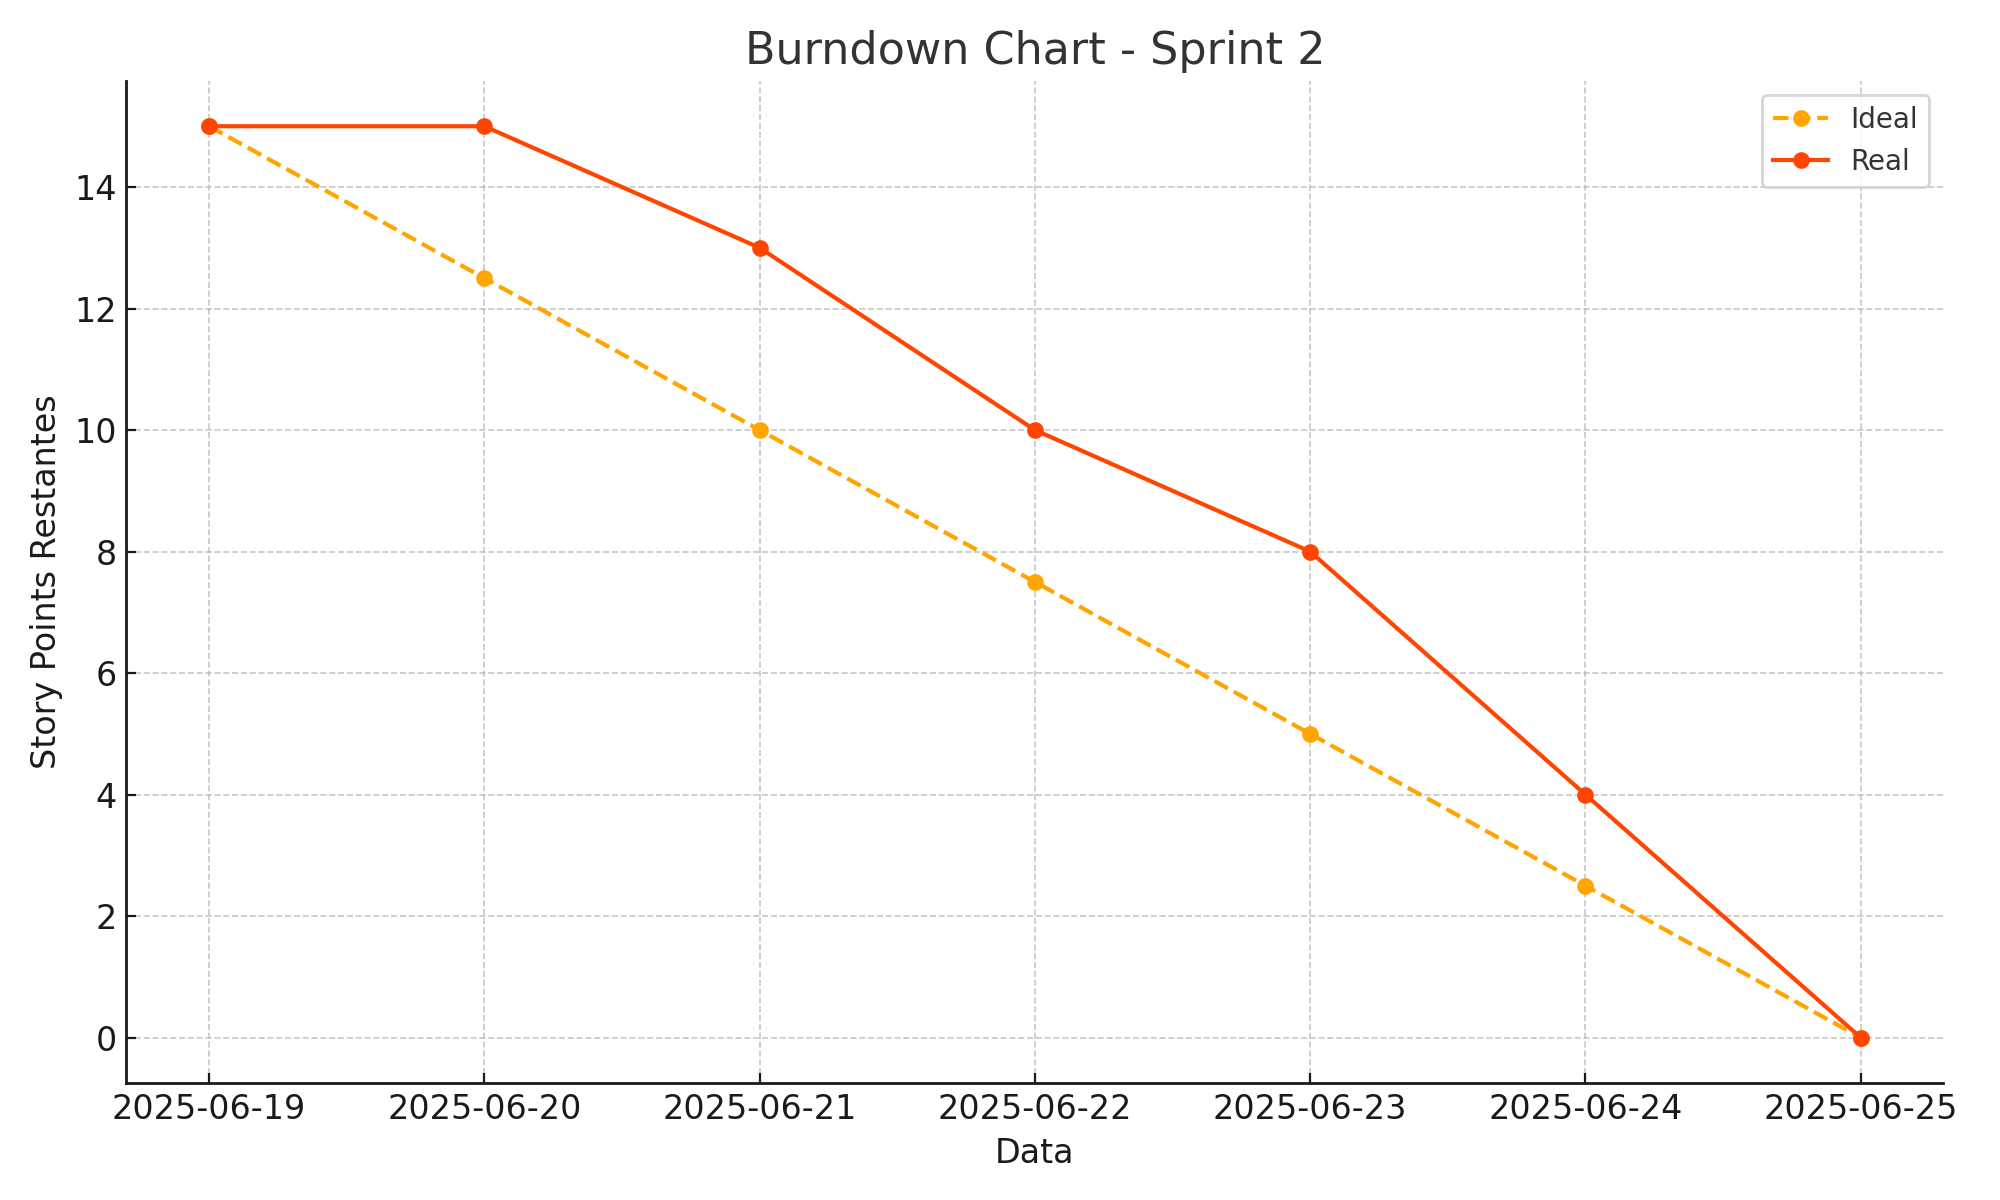
\includegraphics[width=0.8\textwidth]{pictures/burndown_sprint2.png}
\end{center}
